%%%%%%%%%%%%%%%%%%%%%%%%%%%%%%%%%%%%%%%%%
% Beamer Presentation
% LaTeX Template
% Version 1.0 (10/11/12)
%
% This template has been downloaded from:
% http://www.LaTeXTemplates.com
%
% License:
% CC BY-NC-SA 3.0 (http://creativecommons.org/licenses/by-nc-sa/3.0/)
%
%%%%%%%%%%%%%%%%%%%%%%%%%%%%%%%%%%%%%%%%%

%----------------------------------------------------------------------------------------
%	PACKAGES AND THEMES
%----------------------------------------------------------------------------------------

\documentclass{beamer}

\mode<presentation> {

% The Beamer class comes with a number of default slide themes
% which change the colors and layouts of slides. Below this is a list
% of all the themes, uncomment each in turn to see what they look like.

% \usetheme{default}
% \usetheme{AnnArbor}
% \usetheme{Antibes}
% \usetheme{Bergen}
% \usetheme{Berkeley}
%\usetheme{Berlin}
%\usetheme{Boadilla}
%\usetheme{CambridgeUS}
%\usetheme{Copenhagen}
%\usetheme{Darmstadt}
%\usetheme{Dresden}
%\usetheme{Frankfurt}
%\usetheme{Goettingen}
%\usetheme{Hannover}
%\usetheme{Ilmenau}
%\usetheme{JuanLesPins}
%\usetheme{Luebeck}
\usetheme{Madrid}
%\usetheme{Malmoe}
%\usetheme{Marburg}
%\usetheme{Montpellier}
%\usetheme{PaloAlto}
%\usetheme{Pittsburgh}
%\usetheme{Rochester}
%\usetheme{Singapore}
%\usetheme{Szeged}
%\usetheme{Warsaw}

% As well as themes, the Beamer class has a number of color themes
% for any slide theme. Uncomment each of these in turn to see how it
% changes the colors of your current slide theme.

%\usecolortheme{albatross}
%\usecolortheme{beaver}
%\usecolortheme{beetle}
%\usecolortheme{crane}
%\usecolortheme{dolphin}
%\usecolortheme{dove}
%\usecolortheme{fly}
%\usecolortheme{lily}
%\usecolortheme{orchid}
%\usecolortheme{rose}
%\usecolortheme{seagull}
%\usecolortheme{seahorse}
%\usecolortheme{whale}
%\usecolortheme{wolverine}

%\setbeamertemplate{footline} % To remove the footer line in all slides uncomment this line
%\setbeamertemplate{footline}[page number] % To replace the footer line in all slides with a simple slide count uncomment this line

%\setbeamertemplate{navigation symbols}{} % To remove the navigation symbols from the bottom of all slides uncomment this line
}

\usepackage{graphicx} % Allows including images
\usepackage{booktabs} % Allows the use of \toprule, \midrule and \bottomrule in tables
\usepackage{subfigure}
\usepackage[backend=bibtex,sorting=none]{biblatex}
\addbibresource{reference.bib} 
\setbeamerfont{footnote}{size=\tiny}

%----------------------------------------------------------------------------------------
%	TITLE PAGE
%----------------------------------------------------------------------------------------

\title[PhD interview]{PhD Interview} % The short title appears at the bottom of every slide, the full title is only on the title page

\author{Zhaolin Wang} % Your name
\institute[Imperial] % Your institution as it will appear on the bottom of every slide, may be shorthand to save space
{
Imperial College London \\ % Your institution for the title page
\medskip
\textit{zhaolin.wang20@imeprial.ac.uk} % Your email address
}
\date{\today} % Date, can be changed to a custom date

\AtBeginSection[]
{
  \begin{frame}
    \frametitle{Overview} 
    \tableofcontents[currentsection] 
  \end{frame}
}


\begin{document}

\begin{frame}
\titlepage % Print the title page as the first slide
\end{frame}

% \begin{frame}
% \frametitle{Overview} 
% \tableofcontents[currentsection] 
% \end{frame}

%----------------------------------------------------------------------------------------
%	PRESENTATION SLIDES
%----------------------------------------------------------------------------------------

%------------------------------------------------
\section{Background}
\subsection{Education background}
\begin{frame}
\frametitle{Education background}

\begin{block}{Education}

  \begin{minipage}[t]{0.77\textwidth}
    \flushleft{\textbf{Beijing University of Posts and Telecommunications}\footnotemark[1]}
  \end{minipage}
    ~
  \begin{minipage}[t]{0.2\textwidth}
    \flushright{2016 -- 2020}
  \end{minipage}

  {\small \textit{BEng Telecommunications Engineering with Management}} \\

  \begin{minipage}[t]{0.77\textwidth}
    \flushleft{\textbf{Queen Mary University of London}\footnotemark[1]}
  \end{minipage}
    ~
  \begin{minipage}[t]{0.2\textwidth}
    \flushright{2016 -- 2020}
  \end{minipage}
  
  {\small \textit{BEng Telecommunications Engineering with Management, First Class Honours}} \\

  \begin{minipage}[t]{0.77\textwidth}
    \flushleft{\textbf{Imperial College London}}
  \end{minipage}
    ~
  \begin{minipage}[t]{0.2\textwidth}
    \flushright{2020 -- 2021}
  \end{minipage}
  
  {\small \textit{MSc Communications and Signal Processing}} \\

  \footnotetext{\tiny 1. A joint programme of BUPT and QMUL}

\end{block}

\end{frame}
\subsection{Awards}
\begin{frame}
\frametitle{Awards}

\begin{block}{Main Awards}
\begin{itemize}
  \small
  \item Outstanding Final Project Paper of BUPT (Top 2\%)
  \item Outstanding Graduate of BUPT (Top 5\%)
  \item Outstanding Graduate of Beijing (Top 2\%)
  \item First Prize of BUPT Innovation and Entrepreneurship Project (Top 3\%)
  \item College Prize of QMUL (Top 3\%)
\end{itemize}

\end{block}

\end{frame}

\section{Research Experience}
\subsection{Estimate High-fidelity 3D Human Body Models from a Single Image using Deep Learning}

\begin{frame}
    \frametitle{Estimate High-fidelity 3D Human Body Models from a Single Image using Deep Learning}
    \begin{block}{What}
        \small
        An end-to-end framework that can estimate 3D mesh of the human body from a single RGB image.    
    \end{block}
    \begin{figure}
        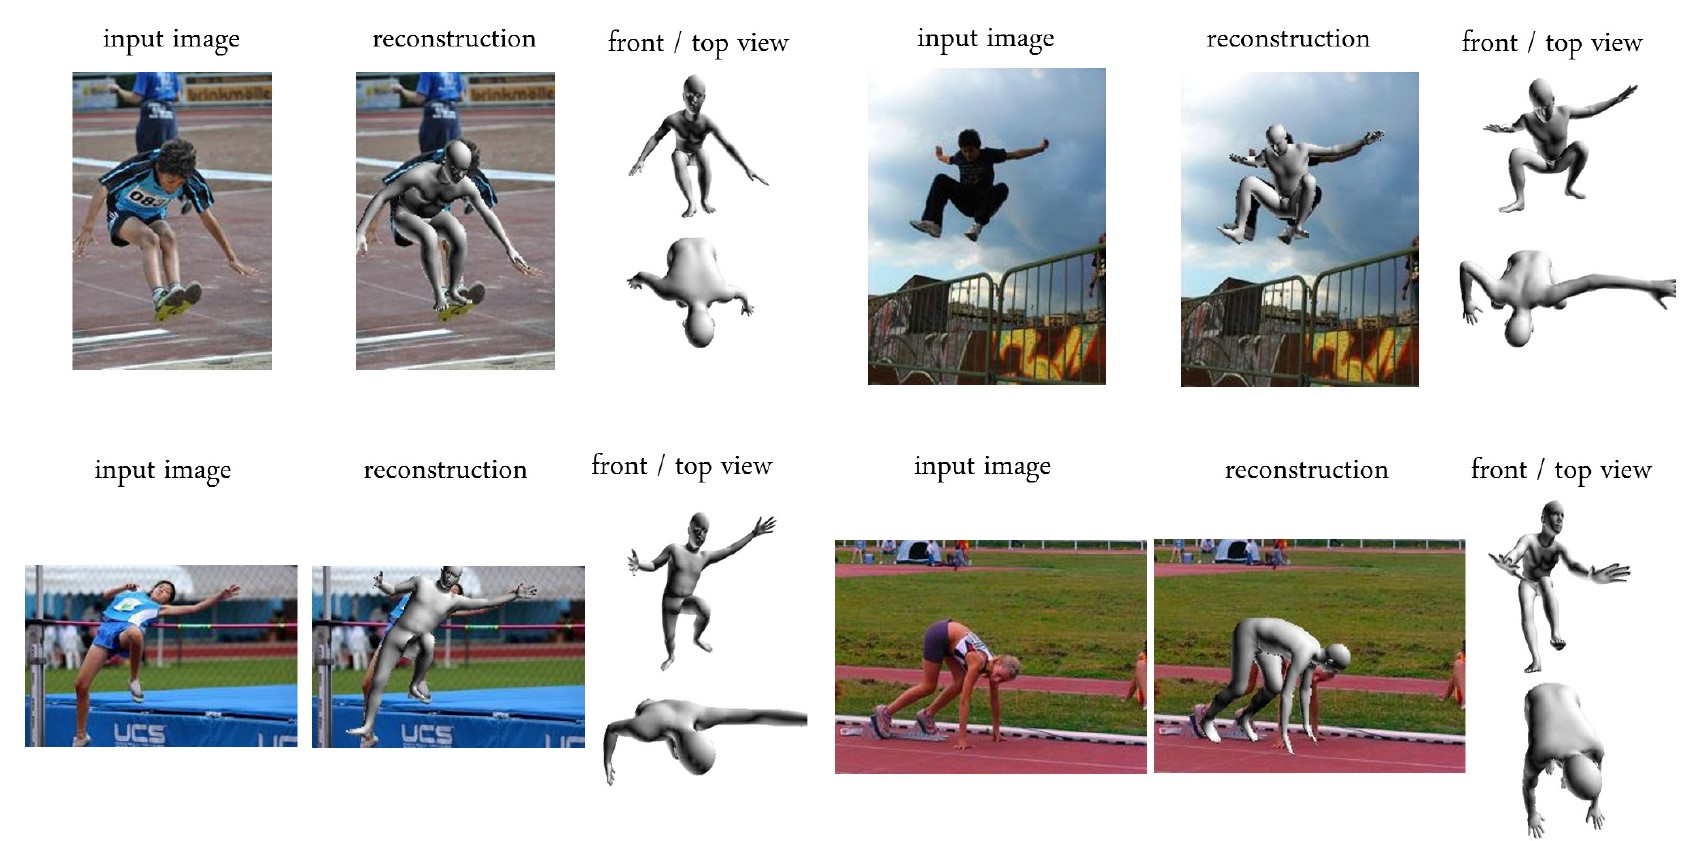
\includegraphics[width=0.8\linewidth]{./img/results_HMR.jpg}
    \end{figure}
\end{frame}

\begin{frame}
    \frametitle{Estimate High-fidelity 3D Human Body Models from a Single Image using Deep Learning}

    \begin{block}{Why}
        \begin{itemize}
        \small
        \item Many existing methods only estimate 3D joints or skeletons (pose), but ignore the 3D shape;
        \item Many existing methods have multiple stages leading to a loss of information;
        \item The lack of in-the-wile images with ground truth 3D annotations.
        \end{itemize}    
    \end{block}

    \begin{block}{How}
        \begin{itemize}
        \small
        \item Apply a skinned multi-person linear (SMPL) model \cite{bogo2016keep} to catch up both 3D pose and shape;
        \item Develop an end-to-end network;
        \item Train the network with a Generative Adversarial Network (GAN) \cite{mirza2014conditional};
        \item Train the network in an iterative error feedback manner (IEF) \cite{carreira2016human}.
        \end{itemize}    
    \end{block}
\end{frame}

\begin{frame}
    \frametitle{Estimate High-fidelity 3D Human Body Models from a Single Image using Deep Learning}
    \begin{itemize}
        \item Framework
        \begin{figure}
            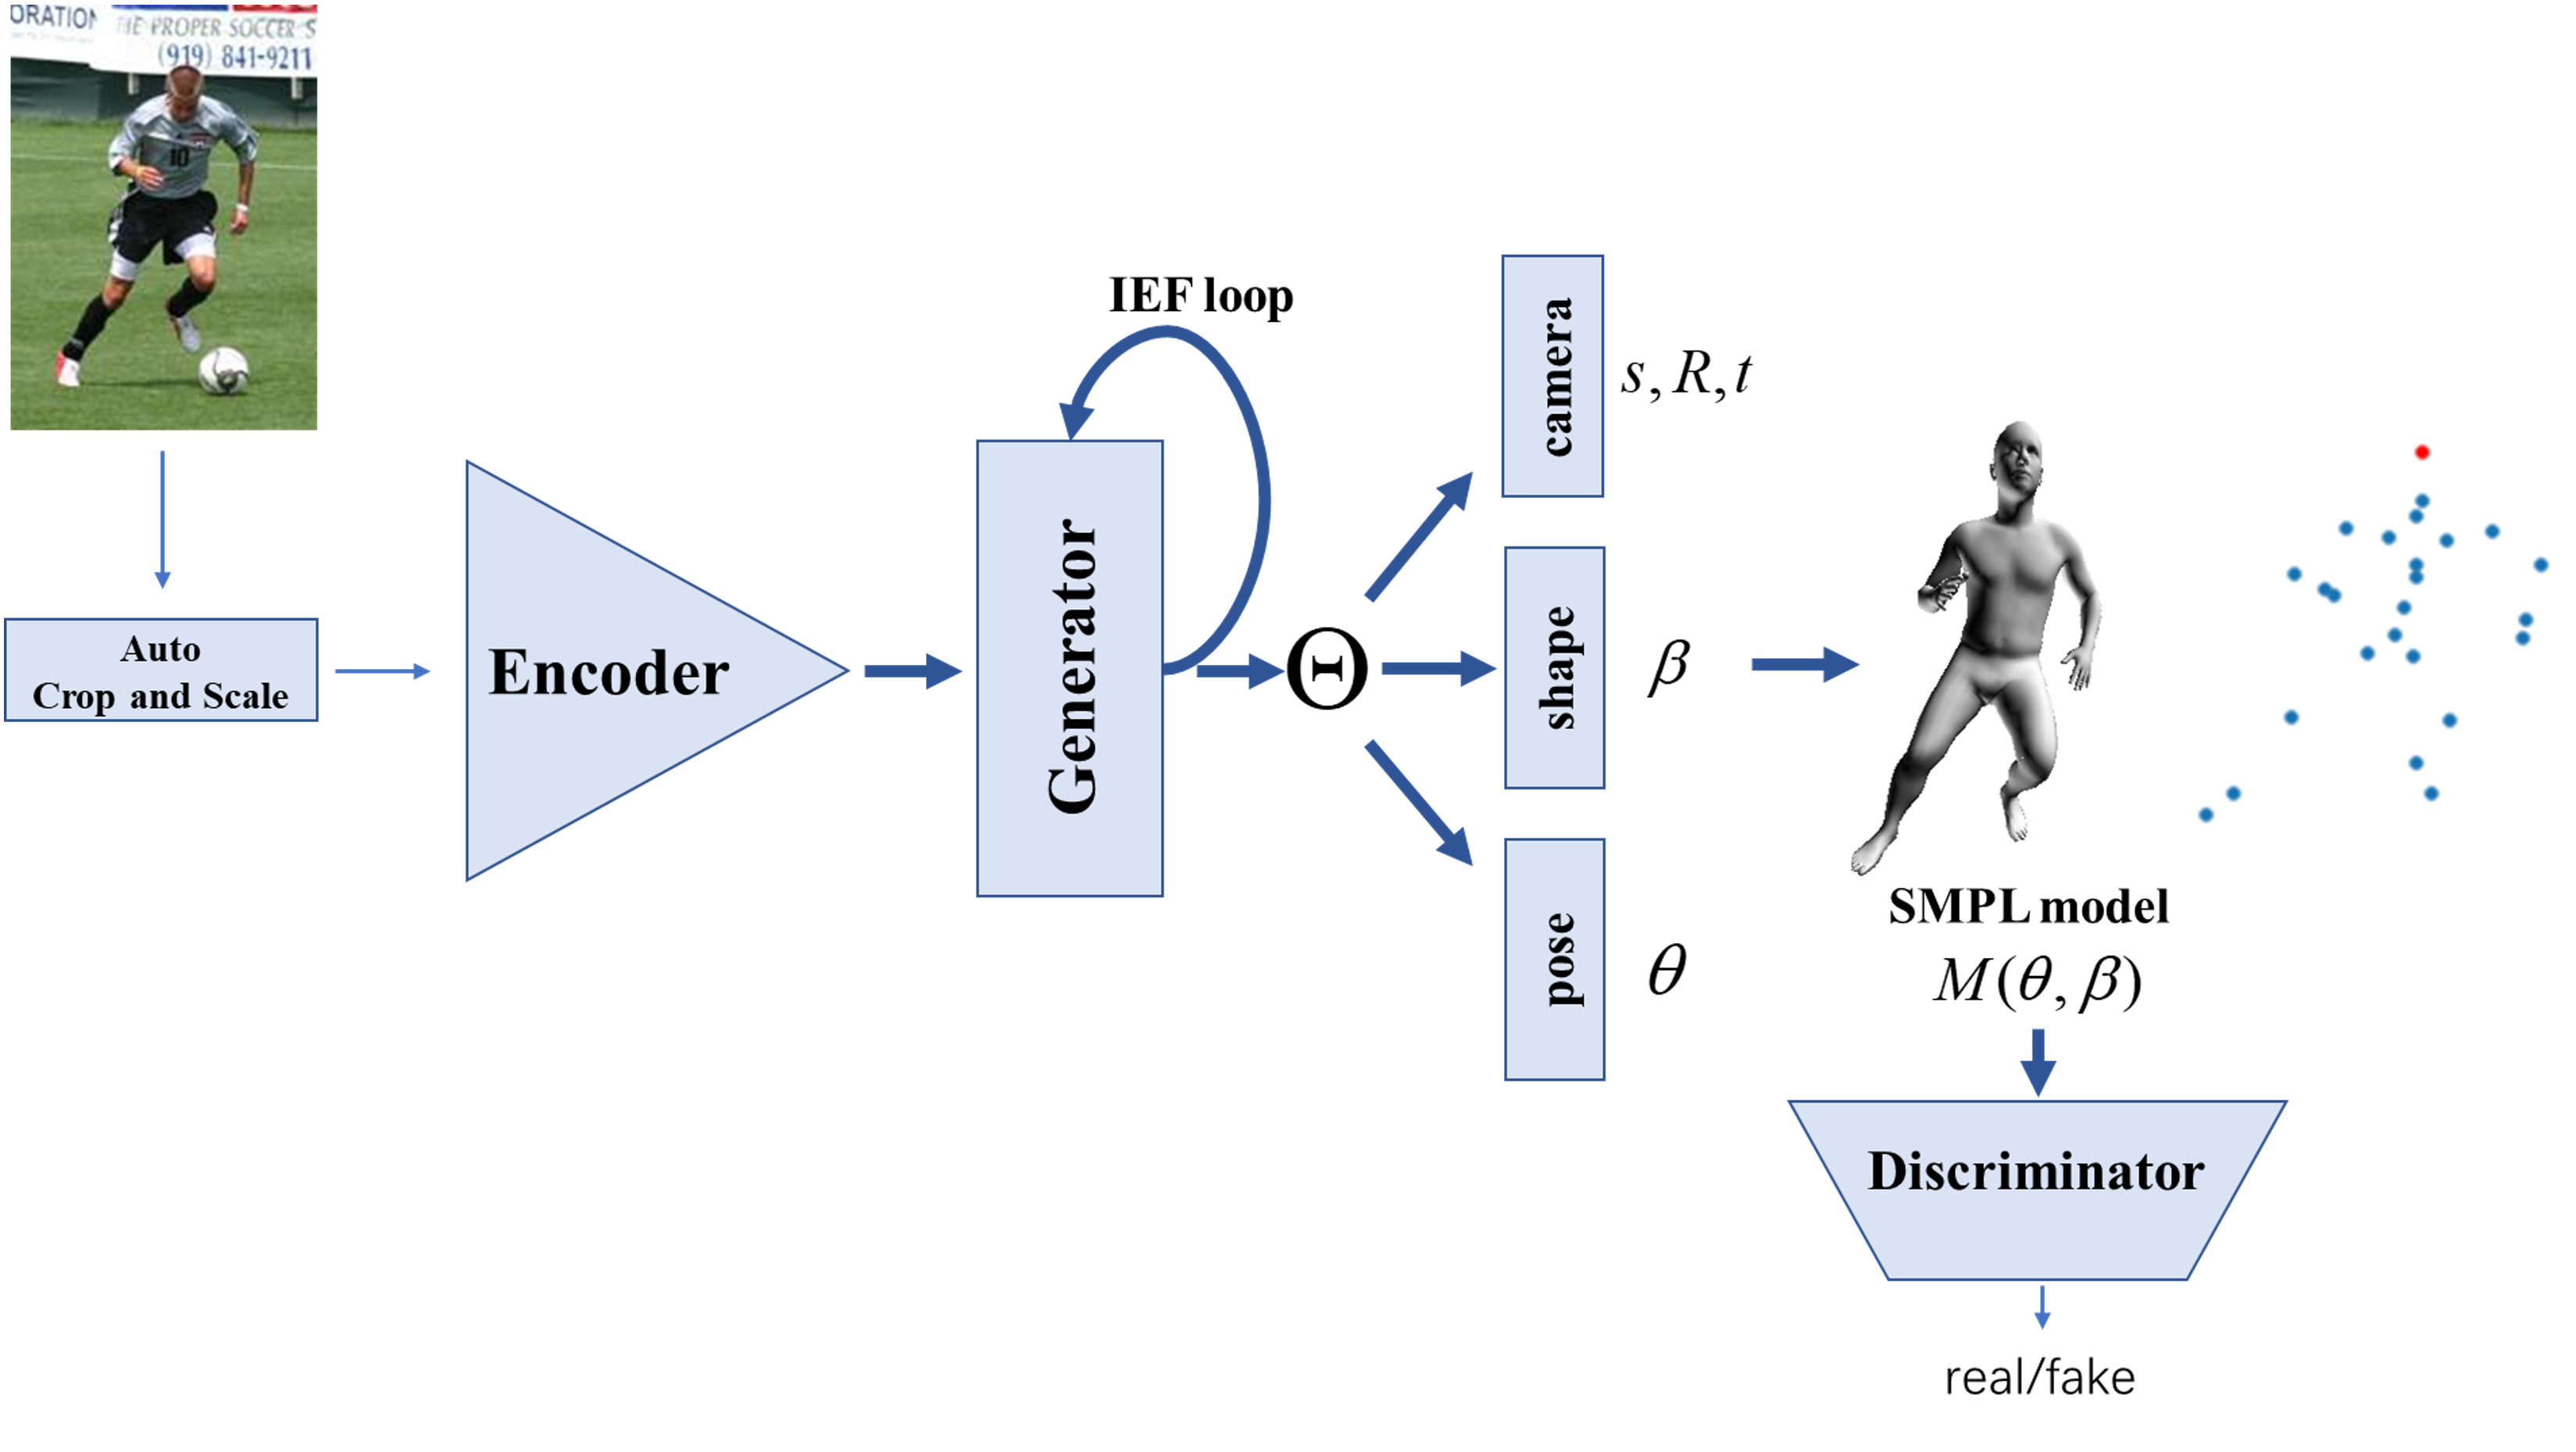
\includegraphics[width=1.0\linewidth]{./img/framework_HMR.png}
        \end{figure}
    \end{itemize}
\end{frame}

\begin{frame}
    \frametitle{Estimate High-fidelity 3D Human Body Models from a Single Image using Deep Learning}
    \begin{block}{Conclusion}
        \begin{itemize}
        \small
        \item With GAN, the overall network can be trained without the in-the-wild images with ground truth 3D annotations, but can still perform well on in-the-wild image.
        \item The training of this network only needs the in-the-wild images with ground truth 2D annotations. Thus, it is easier to improve in the future.       
        \item As the network is end-to-end, the 3D model can be generated fast or even in real time.
        \end{itemize}    
    \end{block}
    % \begin{block}{Limitation}
    %     \begin{itemize}
    %     \small
    %     \item Training GAN requires high computing capability and may cost large resources.
    %     \item As the in-the-wild images with 3D annotations are not used, there is a loss of performance in terms of mean square error.
    %     \end{itemize}    
    % \end{block}
\end{frame}

\subsection{RIS-aided Dual-Functional Radar and Communications Beamforming Design}

\begin{frame}
    \frametitle{RIS-aided Dual-Functional Radar and Communications Beamforming Design}
    \begin{block}{What}
        \small
        An integrated radar and communication system that can simultaneously track a target and serve multiple communication users.
        A reconfigurable intelligent surface is deployed to improve the system performance.   
    \end{block}
    \begin{figure}
        \centering
        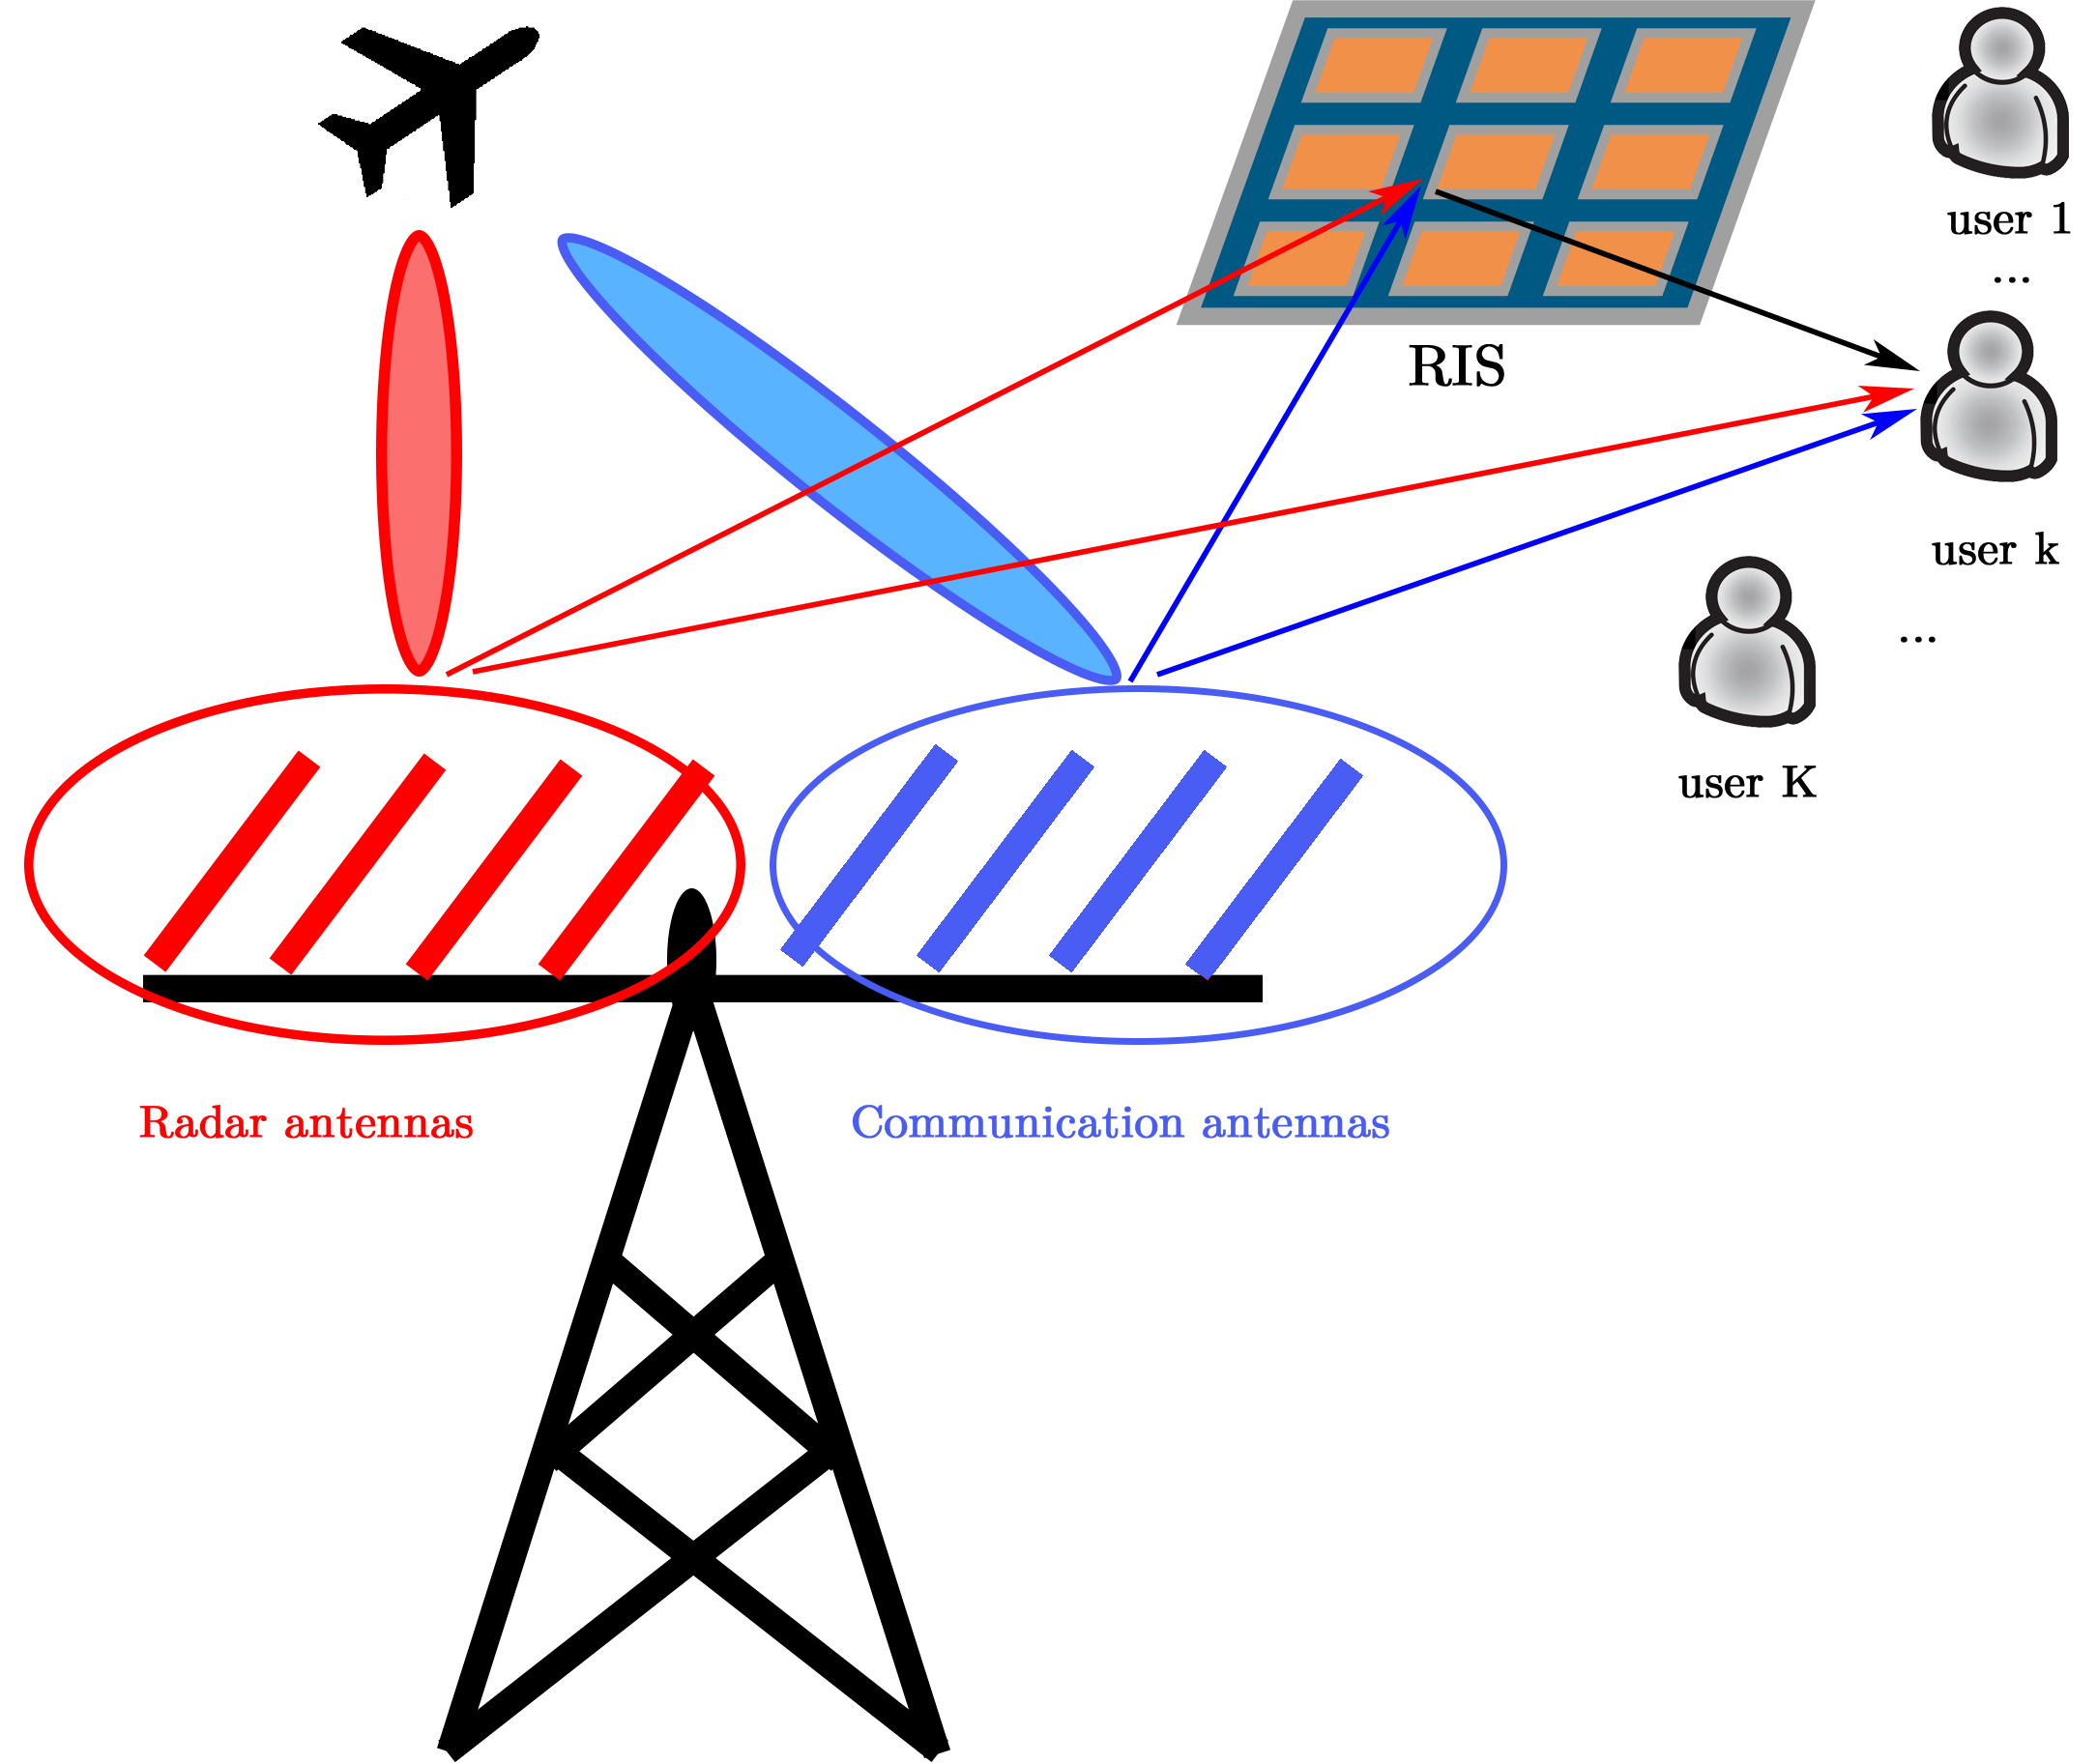
\includegraphics[width=0.4\linewidth]{./img/separated_setup.png}
        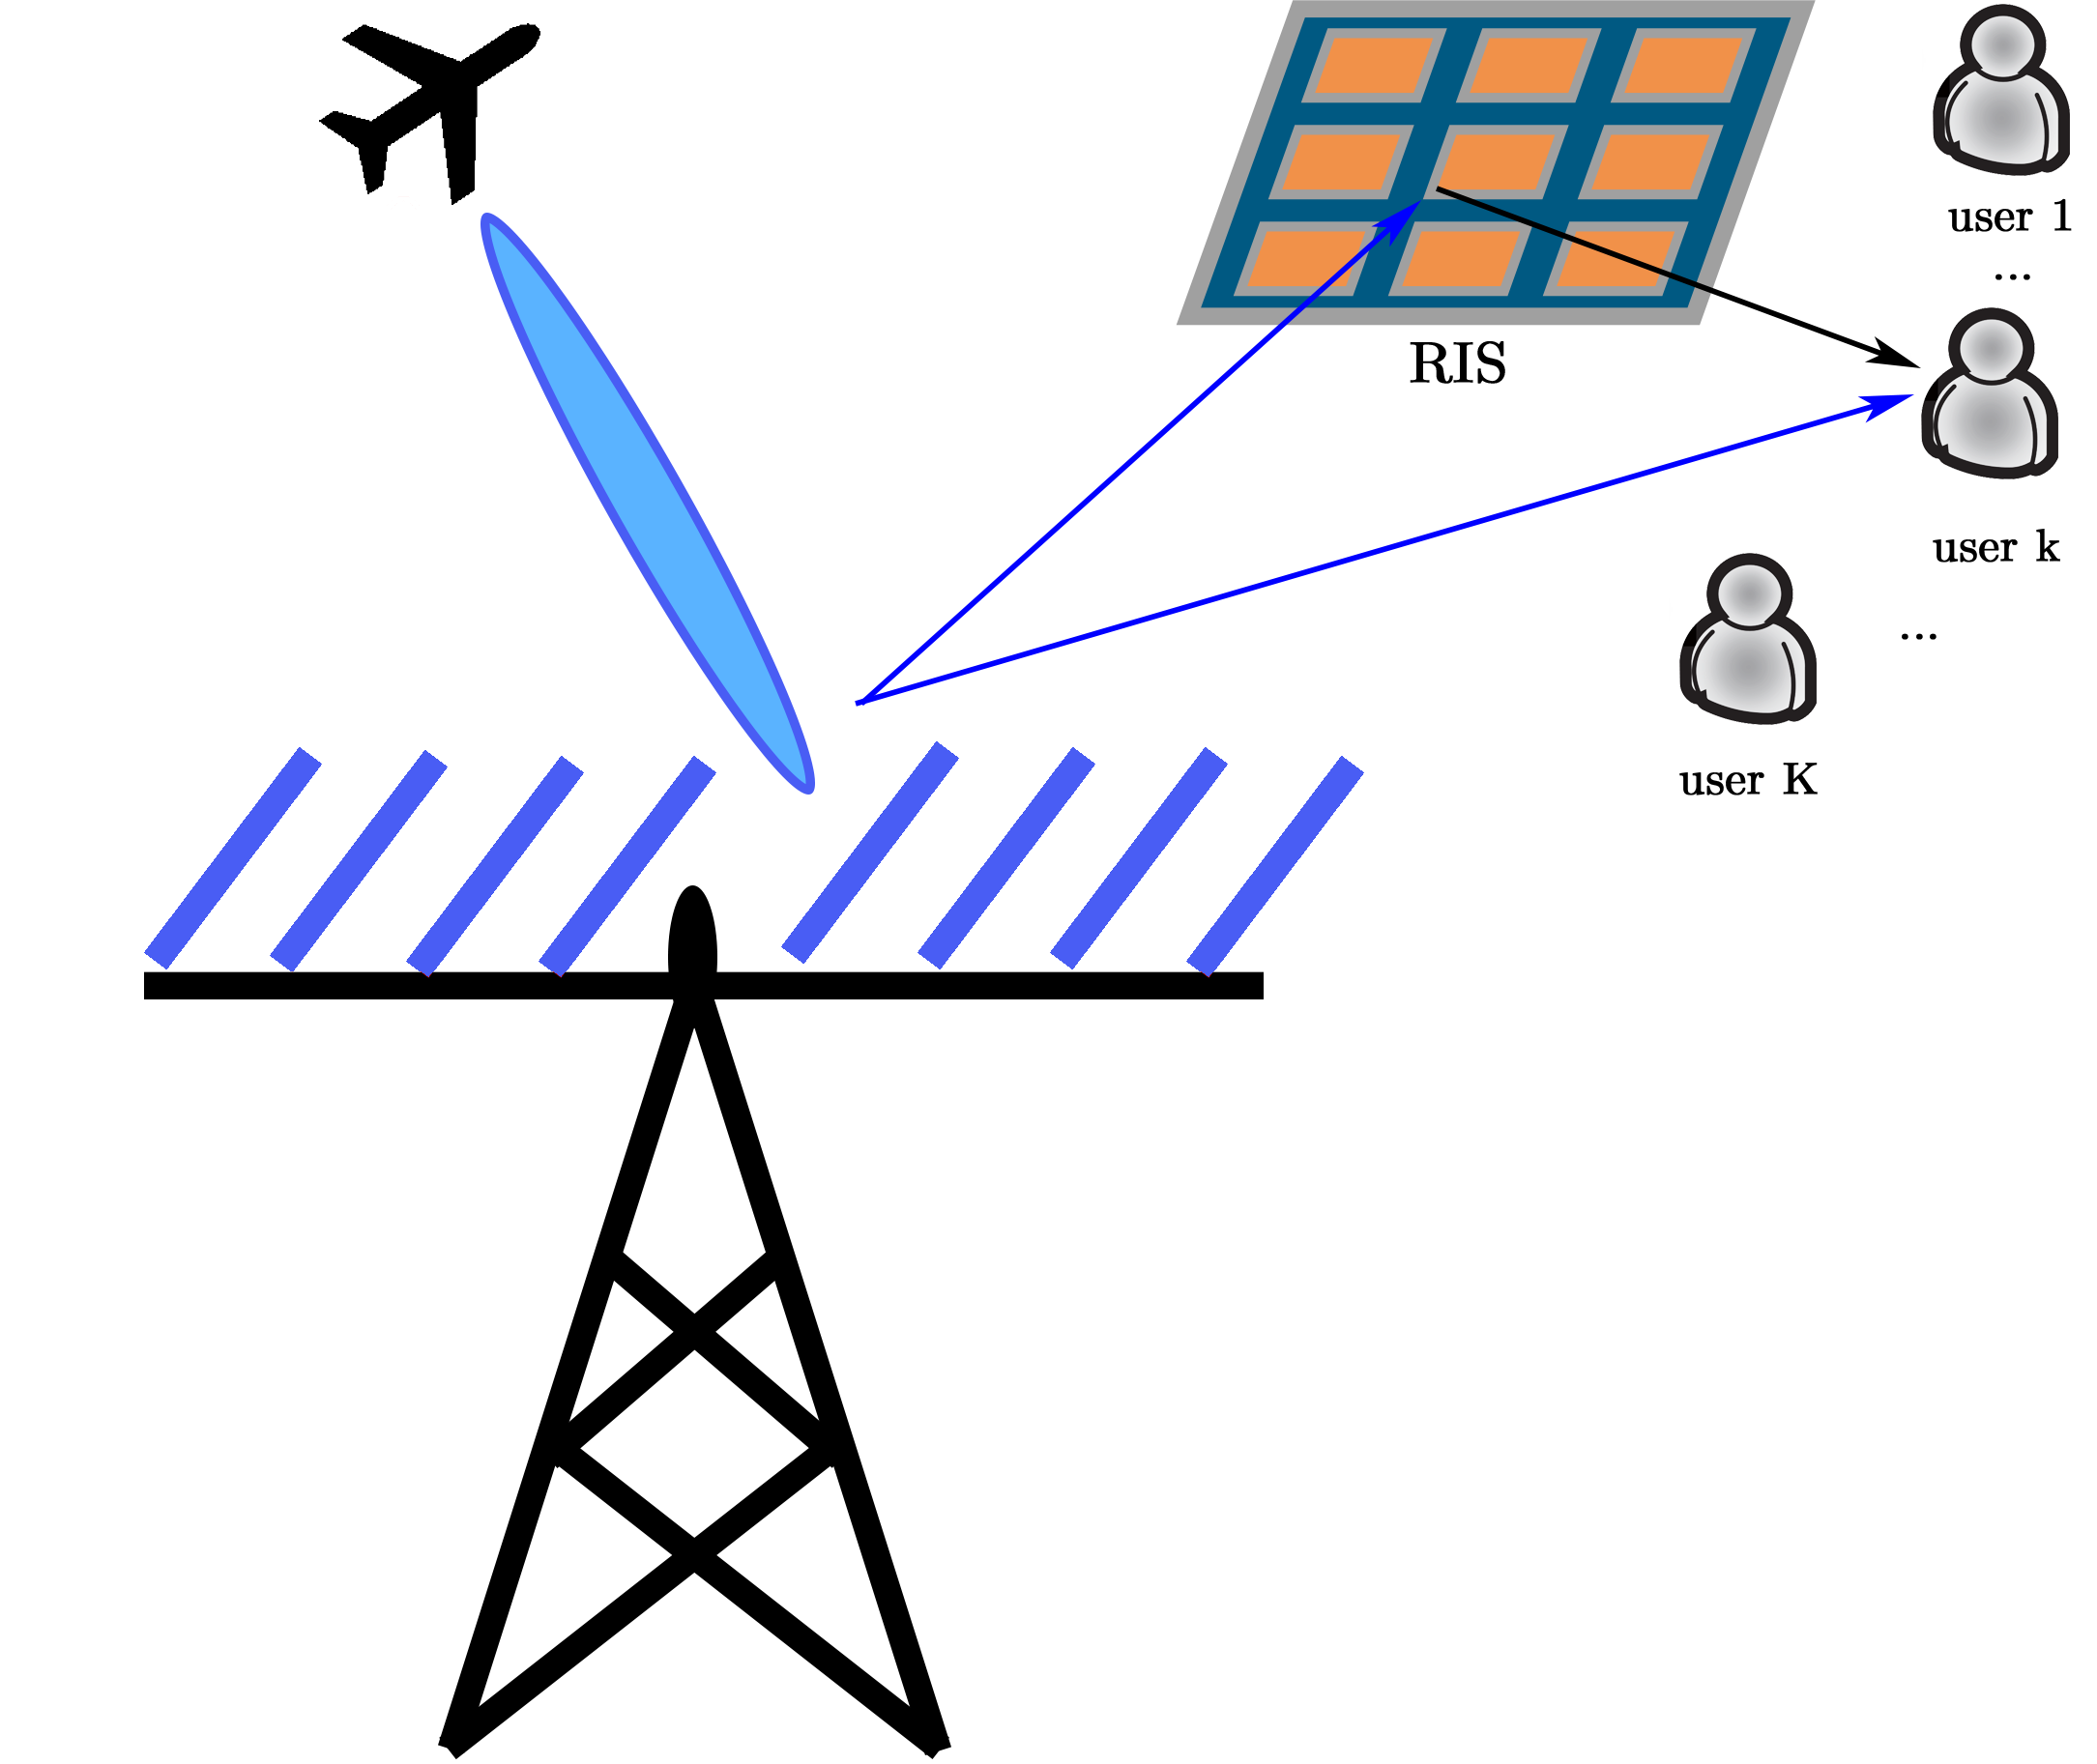
\includegraphics[width=0.4\linewidth]{./img/shared_setup.png}
    \end{figure}
\end{frame}

\begin{frame}
    \frametitle{RIS-aided Dual-Functional Radar and Communications Beamforming Design}

    \begin{block}{Why}
        \begin{itemize}
        \small
        \item To solve the spectrum congestion problem of radar and communication system;
        \item To investigate the benefit of RIS in DFRC system;
        \item Weighted Sum Rate (WSR) maximization has not been studied in RIS-aided DFRC system \cite{wang2020ris, jiang2021dfrc, wang2021joint}.
        \end{itemize}    
    \end{block}

    \begin{block}{How}
        \begin{itemize}
        \small
        \item Jointly design the active and passive beamforming to maximize the WSR and probing power;
        \item Apply a novel group or fully connected RIS model \cite{shen2020modeling};
        \item Simulate the system in both Rayleigh and Rician fading channels.
        \end{itemize}    
    \end{block}
\end{frame}

\begin{frame}
    \frametitle{RIS-aided Dual-Functional Radar and Communications Beamforming Design}
    \tiny
    \begin{figure}
        \centering
        \subfigure[Separated: Rayleigh channel]{
            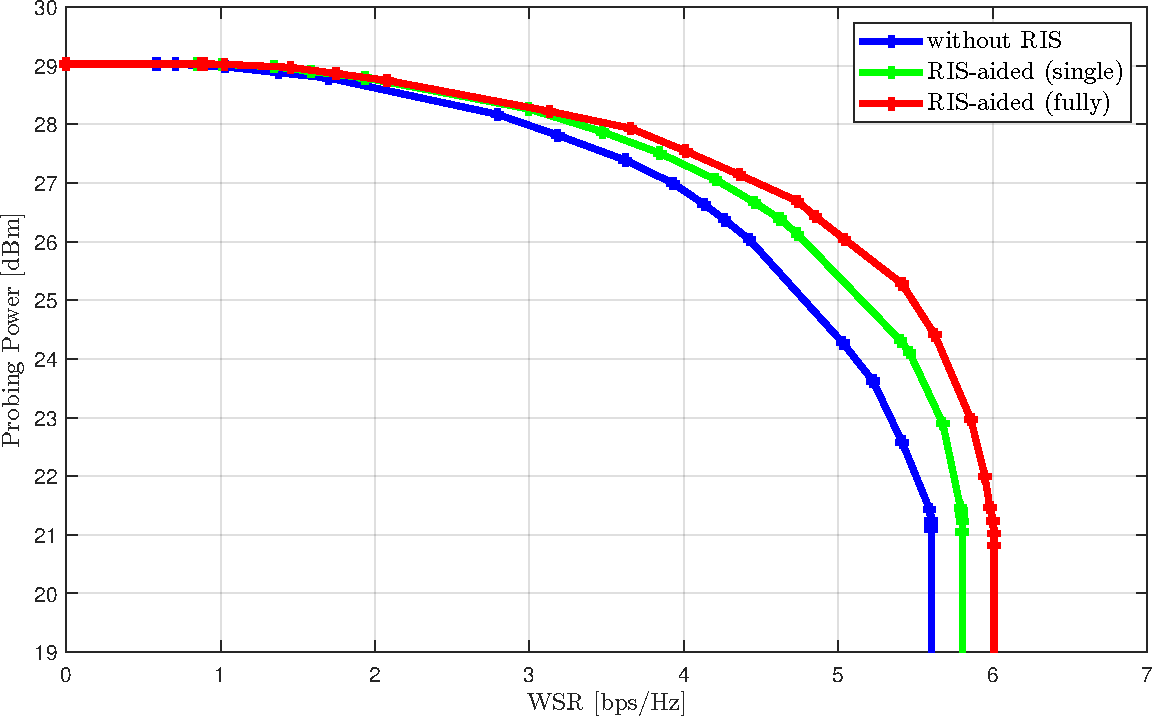
\includegraphics[width=0.4\linewidth]{./img/tradeoff_single_fully_a.pdf}
        }
        \subfigure[Separated: LOS channel]{
        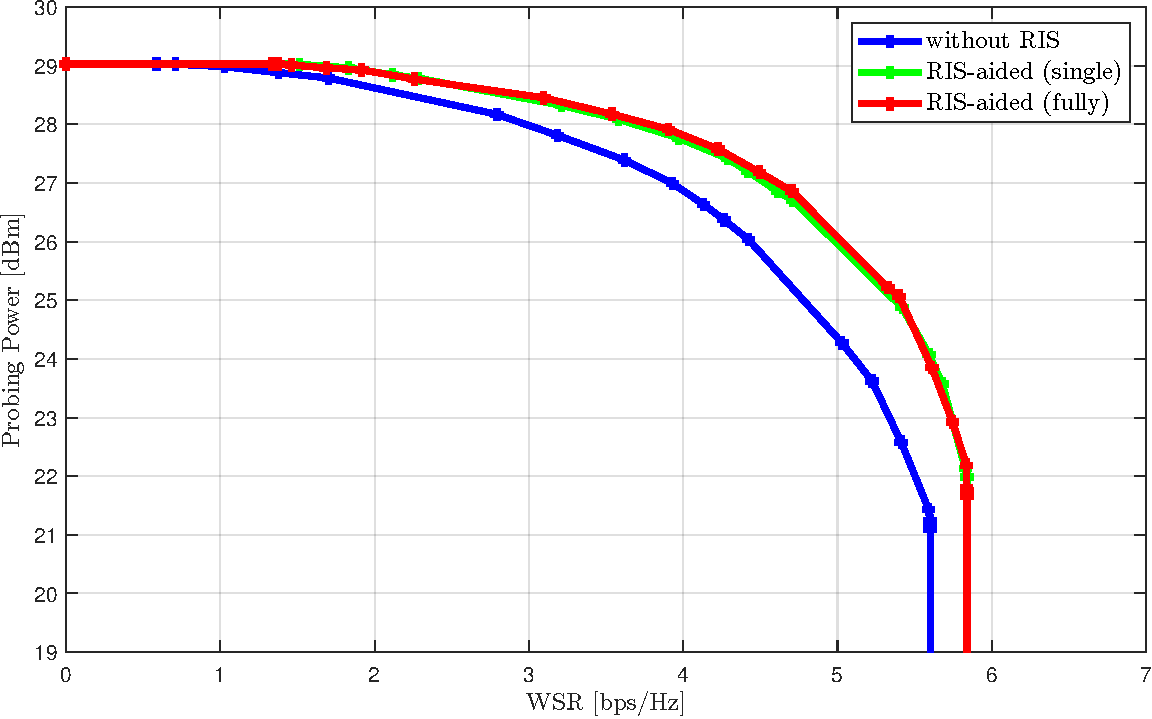
\includegraphics[width=0.4\linewidth]{./img/tradeoff_single_fully_b.pdf}
        }
        \subfigure[Shared: Rayleigh channel]{
            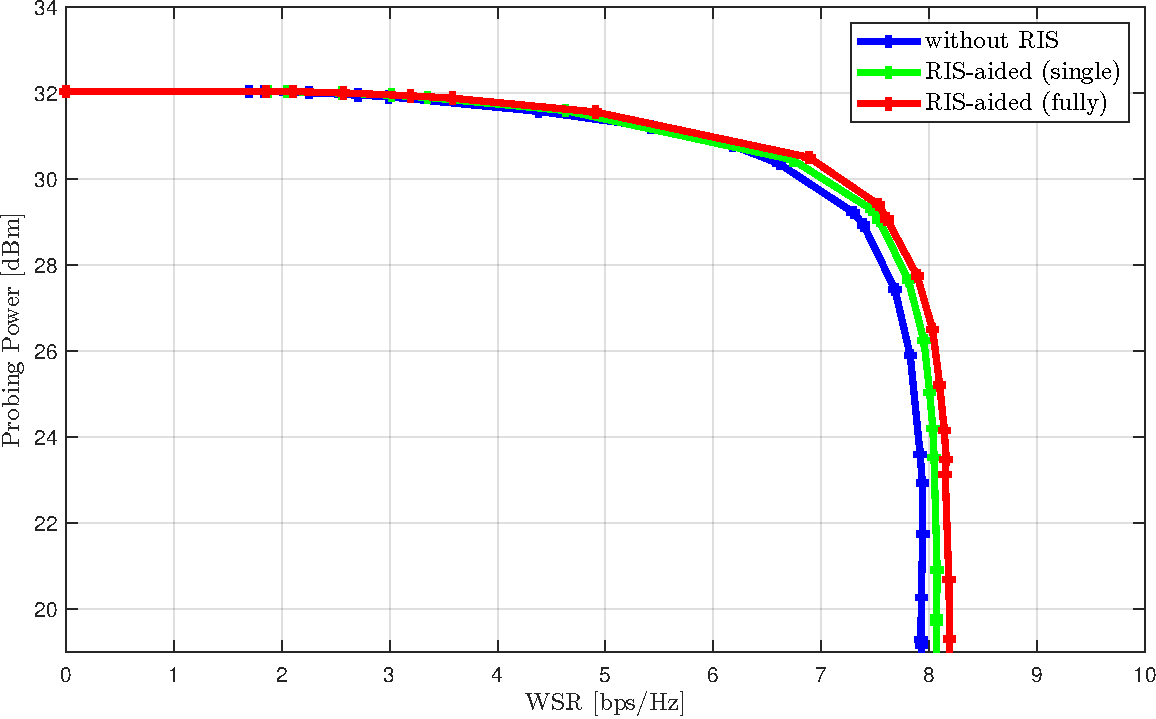
\includegraphics[width=0.4\linewidth]{./img/tradeoff_single_fully_c.pdf}
        }
        \subfigure[Shared: LOS channel]{
        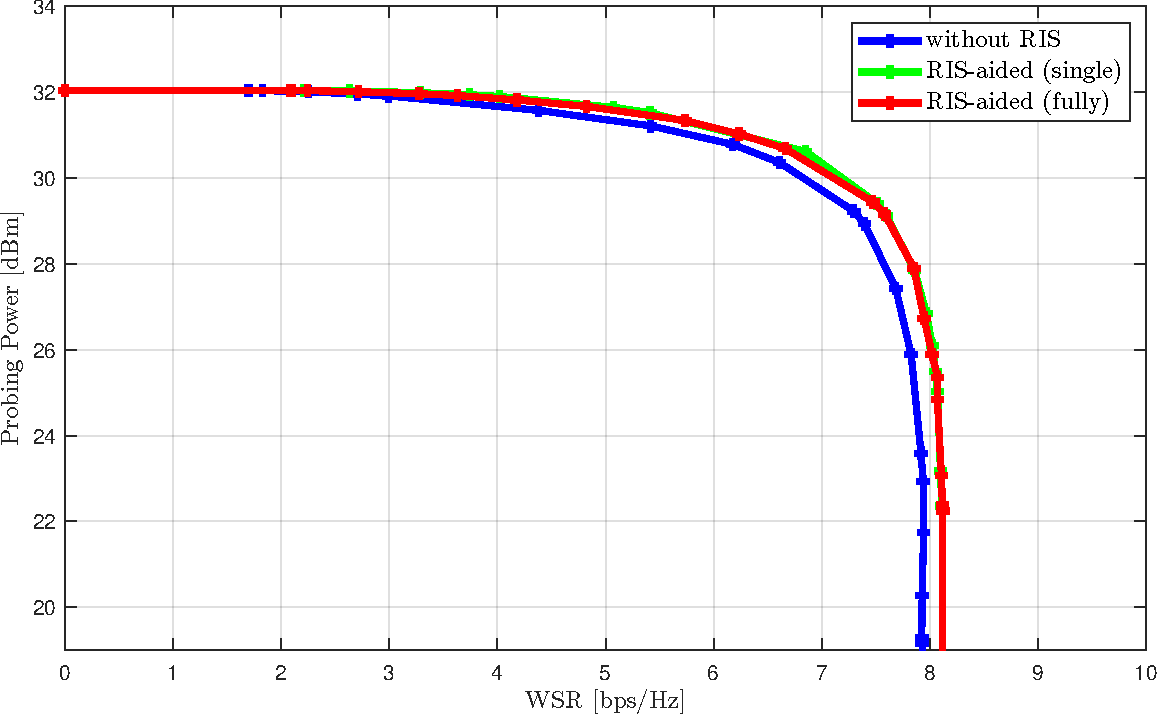
\includegraphics[width=0.4\linewidth]{./img/tradeoff_single_fully_d.pdf}
        }
    \end{figure}
\end{frame}

\begin{frame}
    \frametitle{RIS-aided Dual-Functional Radar and Communications Beamforming Design}
    \begin{figure}
        \centering
        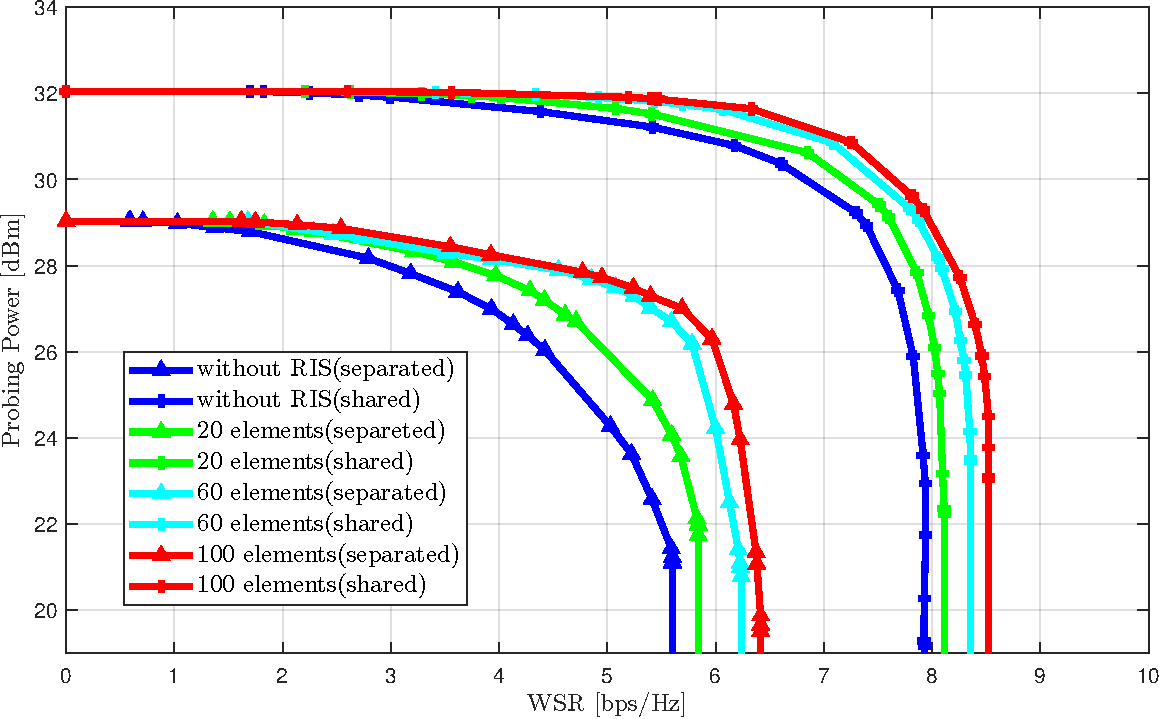
\includegraphics[width=0.7\linewidth]{./img/elements.pdf}
        \caption{Effect of the number of reflecting elements}
    \end{figure}
\end{frame}

\begin{frame}
    \frametitle{Estimate High-fidelity 3D Human Body Models from a Single Image using Deep Learning}
    \begin{block}{Conclusion}
        \begin{itemize}
        \small
        \item RIS is capable of enlarge the achievable region of WSR and probing power.
        \item The fully connected RIS is more powerful than the single connected in Rayleigh channel, but not in LOS channel.        
        \item More gain can be obtained by increasing the reflecting elements.
        \end{itemize}    
    \end{block}
    \begin{block}{Limitation}
        \begin{itemize}
        \small
        \item RIS is only used to improve the communication channel.
        \item The algorithm for the fully connected RIS converges slow. More efficient algorithm need to be found.
        \end{itemize}    
    \end{block}
\end{frame}


\section{Proposal}
\subsection{On Dual-Functional Radar and Communications Design with Reconfigurable Intelligent Surface}
\begin{frame}
    \frametitle{On Dual-Functional Radar and Communications Design with Reconfigurable Intelligent Surface}
    \begin{block}{Motivations}
        \begin{itemize}
        \small
        \item To investigate the benefits of RIS is different system models.
        \item To explore the optimization of conventional radar metrics.
        \item To design more efficient algorithms for RIS-aided DFRC system (try deep learning?). 
        \end{itemize}    
    \end{block}

    \begin{block}{Literatures}
        \begin{itemize}
        \small
        \item Maximize the detection probability under users' SINR constraints in RIS-aided RCC system \cite{wang2020ris}
        \item Maximize the SINR of radar echo signal under users' SINR constraints in RIS-aided DFRC system \cite{jiang2021dfrc}
        \item Minimize the multi-user interference while approximate desired beampattern in RIS-aided DFRC system \cite{wang2021joint}
        \end{itemize}    
    \end{block}
\end{frame}

\begin{frame}
    \frametitle{On Dual-Functional Radar and Communications Design with Reconfigurable Intelligent Surface}
    \begin{block}{No-RIS DFRC vs RIS-aided DFRC}
        \begin{itemize}
        \small
        \item In No-RIS DFRC, radar metric is usually approximating a desired beampattern \cite{liu2018beamforming,liu2020beamforming,xu2020tradeoff}. But we can achieve more if the echo signals are considered in RIS-aided DFRC.
        \end{itemize}    
    \end{block}
    \begin{figure}
        \centering
        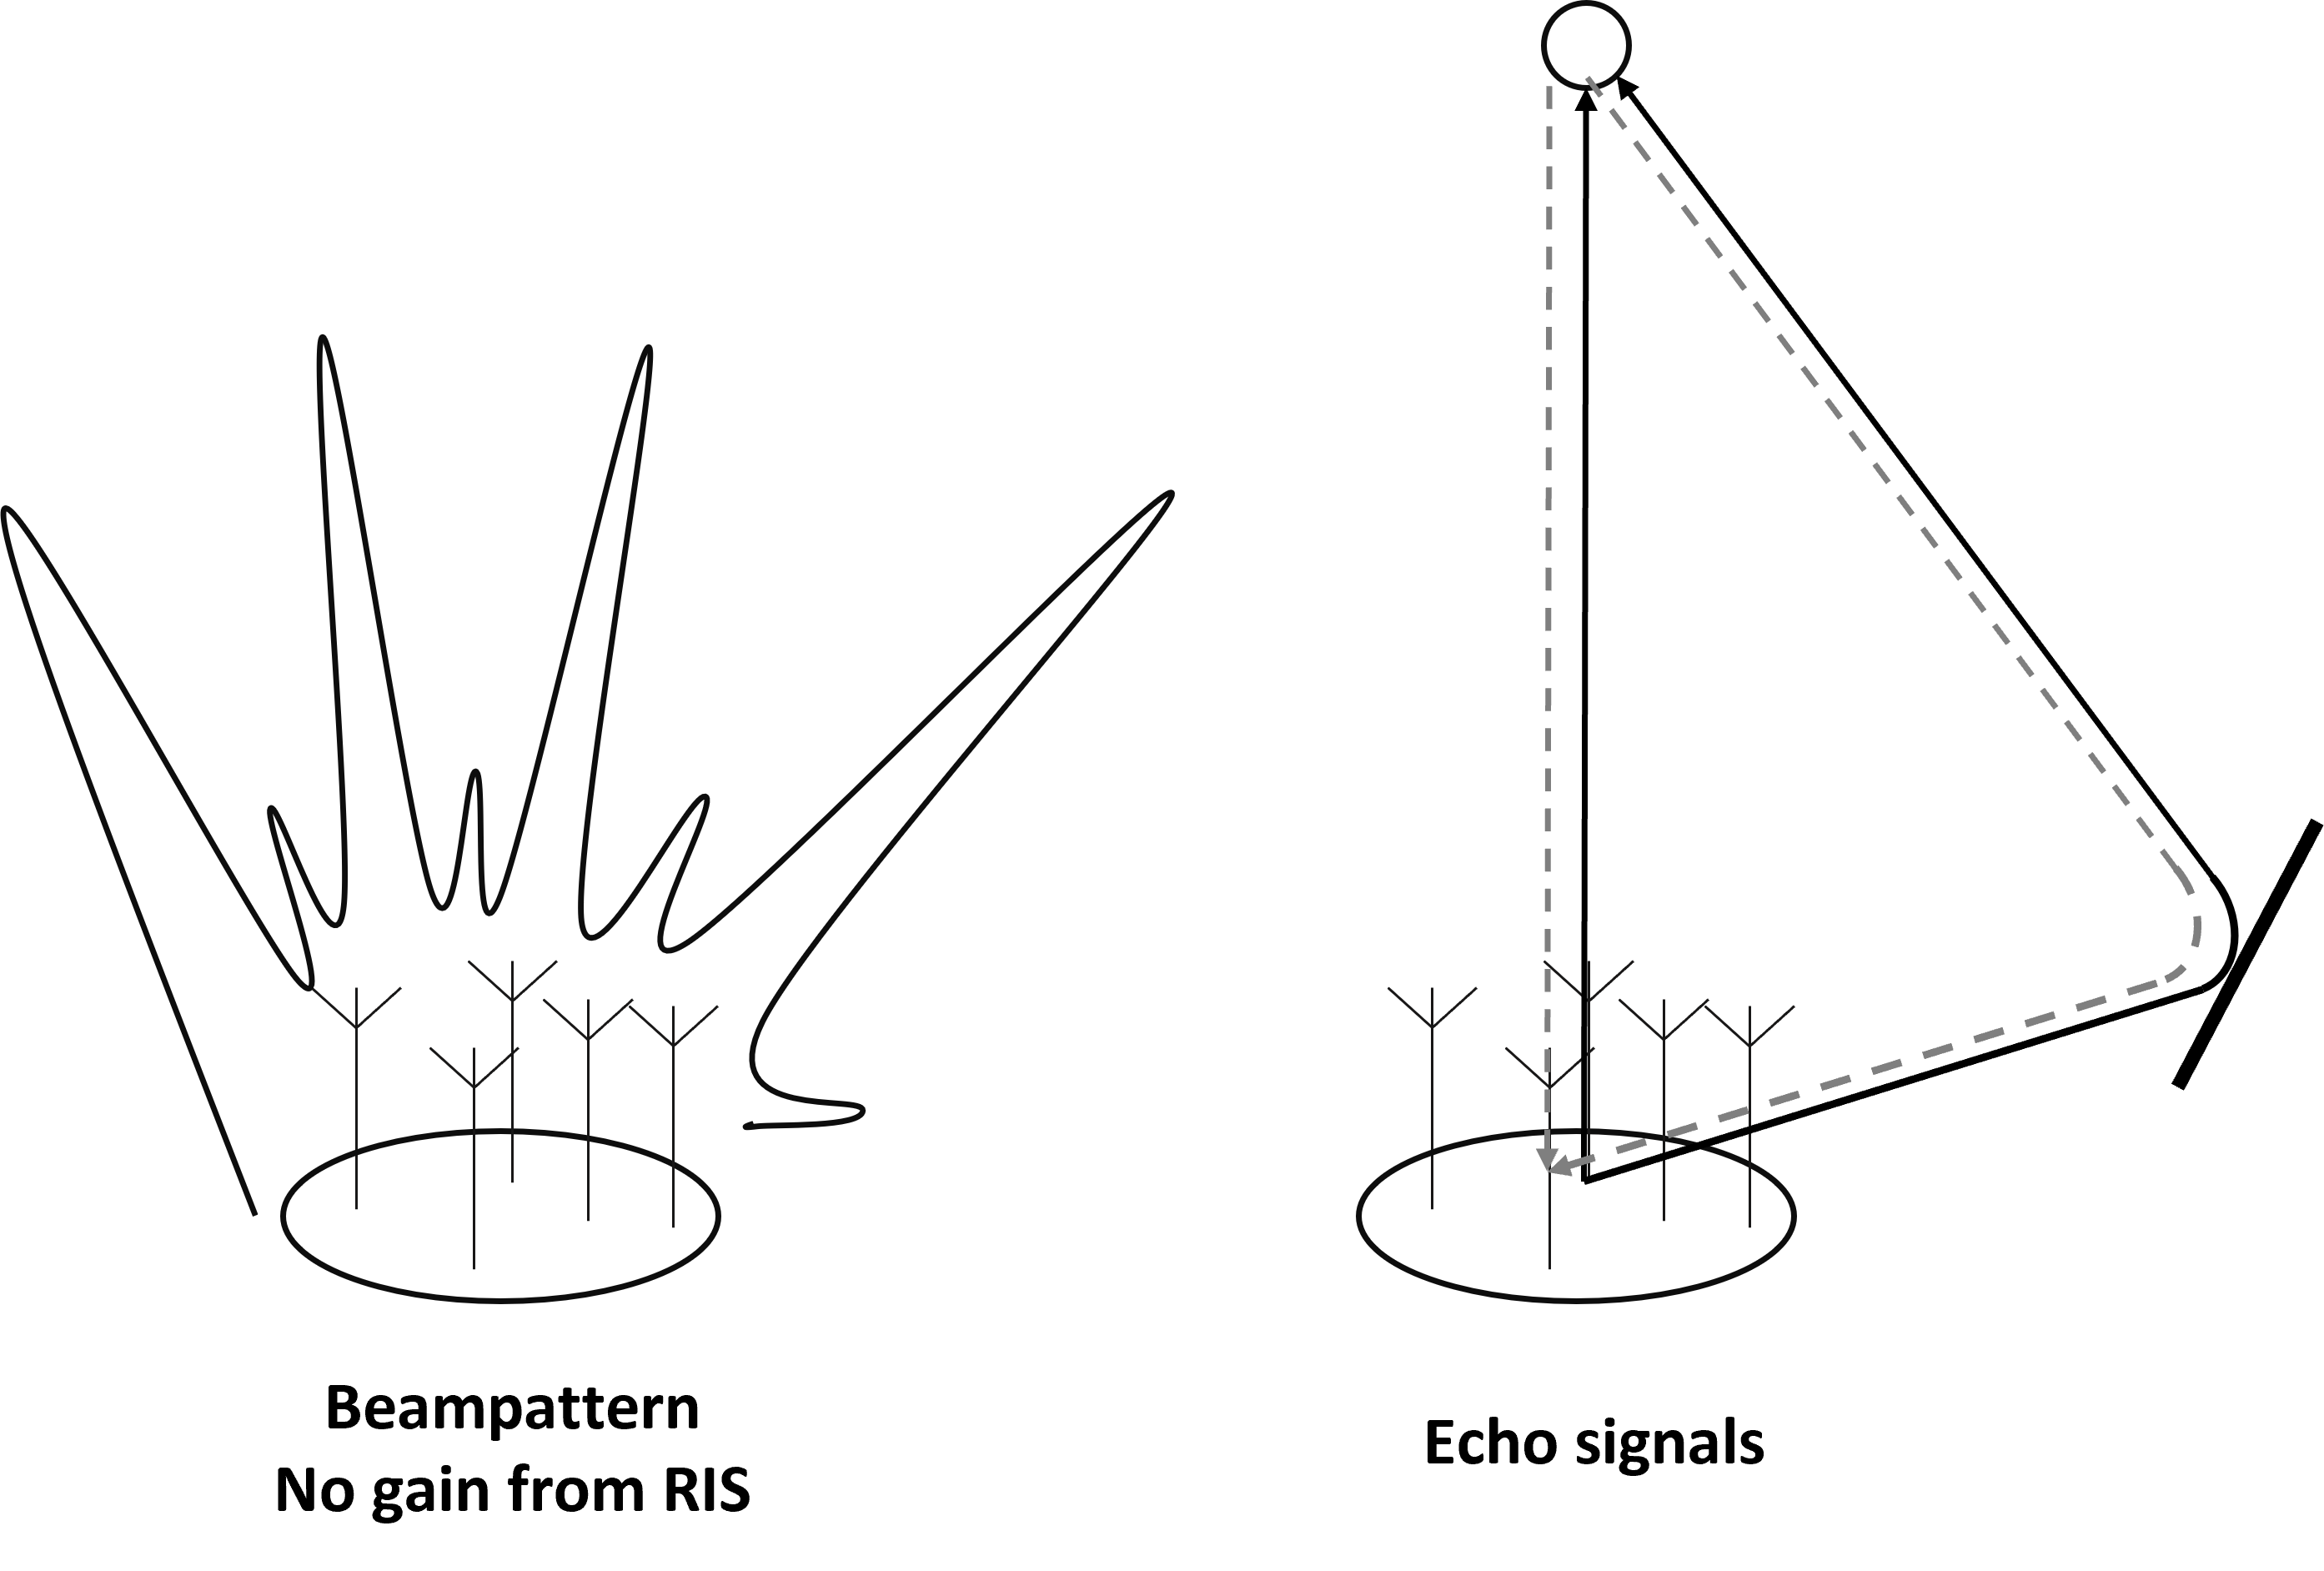
\includegraphics[width=0.6\linewidth]{./img/No-RIS_vs_RIS-aided.png}
    \end{figure}
\end{frame}

\begin{frame}
    \frametitle{On Dual-Functional Radar and Communications Design with Reconfigurable Intelligent Surface}
    \begin{block}{Conventional radar metrics}
        \begin{itemize}
        \small
        \item Detection: detection probability $P_D$ and false-alarm probability $P_{FA}$
        \item Estimation: mean square error
        \end{itemize}    
    \end{block}

    \begin{block}{Example}
        \small
        According to \cite{wang2020ris}, when the generalized likelihood ratio test under the
        Neyman-Pearson criterion is applied, the detection probability is given as
        \begin{equation}
            P_D = 1 - \mathfrak{F}_{\mathcal{X}_2^2(\rho)}\Big(\mathfrak{F}_{\mathcal{X}_2^2}^{-1}(1-P_{FA})\Big)
        \end{equation}
        If the radar signal is orthogonal, i.e., ${\bf R_r}=P_R{\bf I}_{N_t}$, and the echo signal is ${\bf y} = \beta{\bf Cr + z}$, 
        the parameter $\rho$ is
        \begin{equation}
            \rho = |\beta|^2 P_R {\rm Tr}\Big( {\bf CC}^H {\bf R}_{\bf z}^{-1} \Big) \geq {\rm SINR_{echo}}
        \end{equation}
    \end{block}
\end{frame}

\begin{frame}
    \frametitle{On Dual-Functional Radar and Communications Design with Reconfigurable Intelligent Surface}
    \begin{block}{Potential benefits of deep learning}
        \begin{itemize}
        \small
        \item Deep learning may catch up more information than conventional optimization method.
        % \item Deep learning may be helpful to reach the optimal metric without closed form.
        \item Deep learning algorithm may have lower complexity.
        \end{itemize}    
    \end{block}

    \begin{block}{A simple idea}
        \small
        Deep reinforcement learning: we can set the detection probability and WSR as reward, and the model will learn what is the optimal beamforming (actions) in different environments (states).
    \end{block}
\end{frame}



%------------------------------------------------

\begin{frame}[allowframebreaks]{References}
    \printbibliography
\end{frame}

\begin{frame}
  \Huge{\centerline{Thank you}}
\end{frame}

% \frametitle{Reference}
% % {\huge \textbf{Reference}}
% \printbibliography


% \begin{frame}
% 	\bibliographystyle{IEEEtran}
%     \bibliography{reference}
% \end{frame}

% \bibliographystyle{IEEEtran}
% \bibliography{reference}

%----------------------------------------------------------------------------------------

\end{document} 